\section{Introdução}

Esta prática tem como objetivo criar uma semáforo de carros e pedestres,
em que o pedestre pode solicitar sua passagem e um display de 7
segmentos mostra o tempo que ele tem para fazer a passagem. Imagine que
este semáforo está em uma auto estrada de alta velocidade. Nesse cenário
o sinal para os carros está sempre verde e para os pedestres está sempre
vermelho. Quando um pedestre solicita a passagem através de um botão, o
sinal para os carros sai do vermelho para o amarelo, logo em seguida
para o vermelho, enquanto isso o sinal dos pedestres vai para o verde e
um par de displays de 7 segmentos mostra o tempo que o pedestre tem para
passar.

\section{Material}

\begin{itemize}
\item
  5 LEDs
\item
  7 Resistores $390 \Omega$
\item
  2 Displays de 7 segmentos
\item
  1 Cabo USB
\item
  1 Placa SanUSB
\item
  1 Protoboard
\end{itemize}
\section{Iteração 1 - Semáforo simples}

Inicialmente faremos um semáforo simples apenas dos carros, como mostra
a figura a seguir:

\begin{figure}[h]
    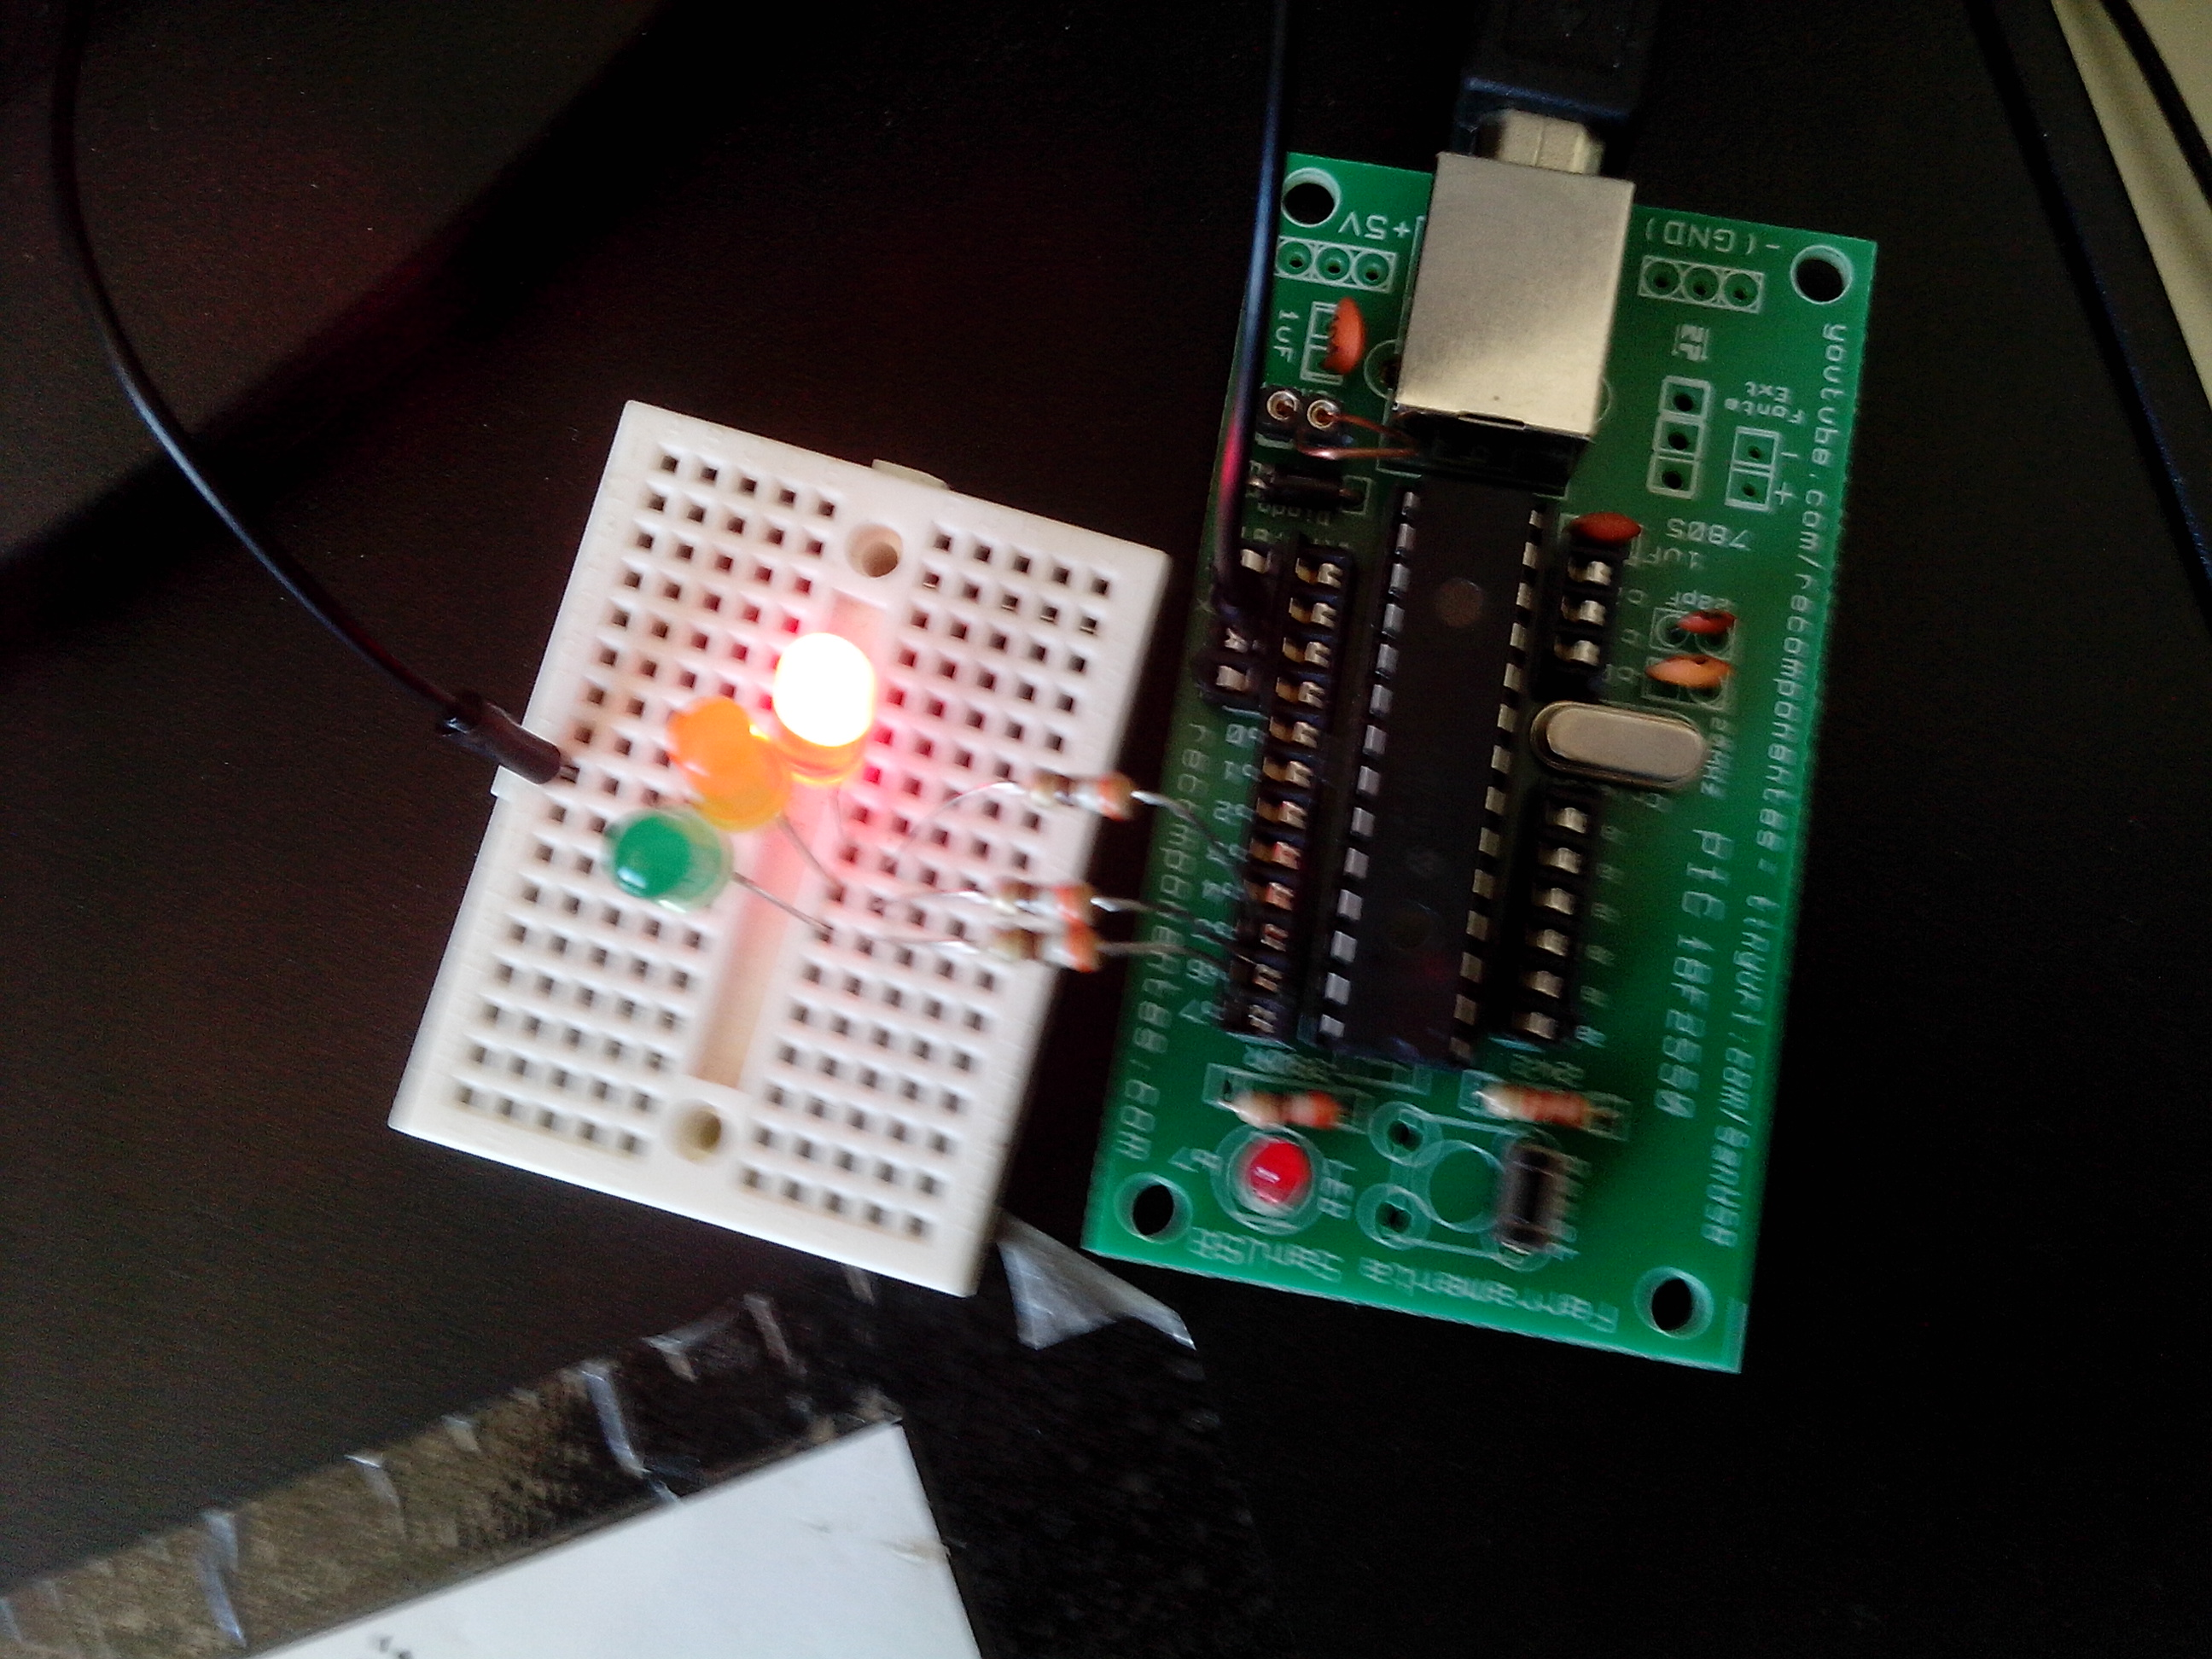
\includegraphics[scale=0.15]{img/semaforo-1.jpg}
    \caption{Semáforo Simples de Carros}
\end{figure}

Segue o código fonte da iteração:

\begin{Shaded}
\begin{Highlighting}[]
\OtherTok{#include "SanUSB48X.h"}

\DataTypeTok{void} \NormalTok{interrupt interrupcao() \{\}}

\DataTypeTok{void} \NormalTok{main(}\DataTypeTok{void}\NormalTok{) \{}
    \NormalTok{clock_int_48MHz();}
    \KeywordTok{while} \NormalTok{(}\DecValTok{1}\NormalTok{) \{}
        \NormalTok{nivel_alto(pin_b7);}
        \NormalTok{tempo_ms(}\DecValTok{3000}\NormalTok{);}
        \NormalTok{nivel_baixo(pin_b7);}

        \NormalTok{nivel_alto(pin_b6);}
        \NormalTok{tempo_ms(}\DecValTok{1000}\NormalTok{);}
        \NormalTok{nivel_baixo(pin_b6);}

        \NormalTok{nivel_alto(pin_b5);}
        \NormalTok{tempo_ms(}\DecValTok{3000}\NormalTok{);}
        \NormalTok{nivel_baixo(pin_b5);}
    \NormalTok{\}}
\NormalTok{\}}
\end{Highlighting}
\end{Shaded}
\newpage

\section{Iteração 2 - Semáforo simples para carros e pedestres}

Em seguida faremos um semáforo tanto para os carros quanto para os
pedestres. O semáforo deve estar sempre verde para os carros e vermelho
para os pedestres. Ao acionar um botão o semáforo entra num processo em
que o sinal alterna por um tempo.

\begin{figure}[H]
    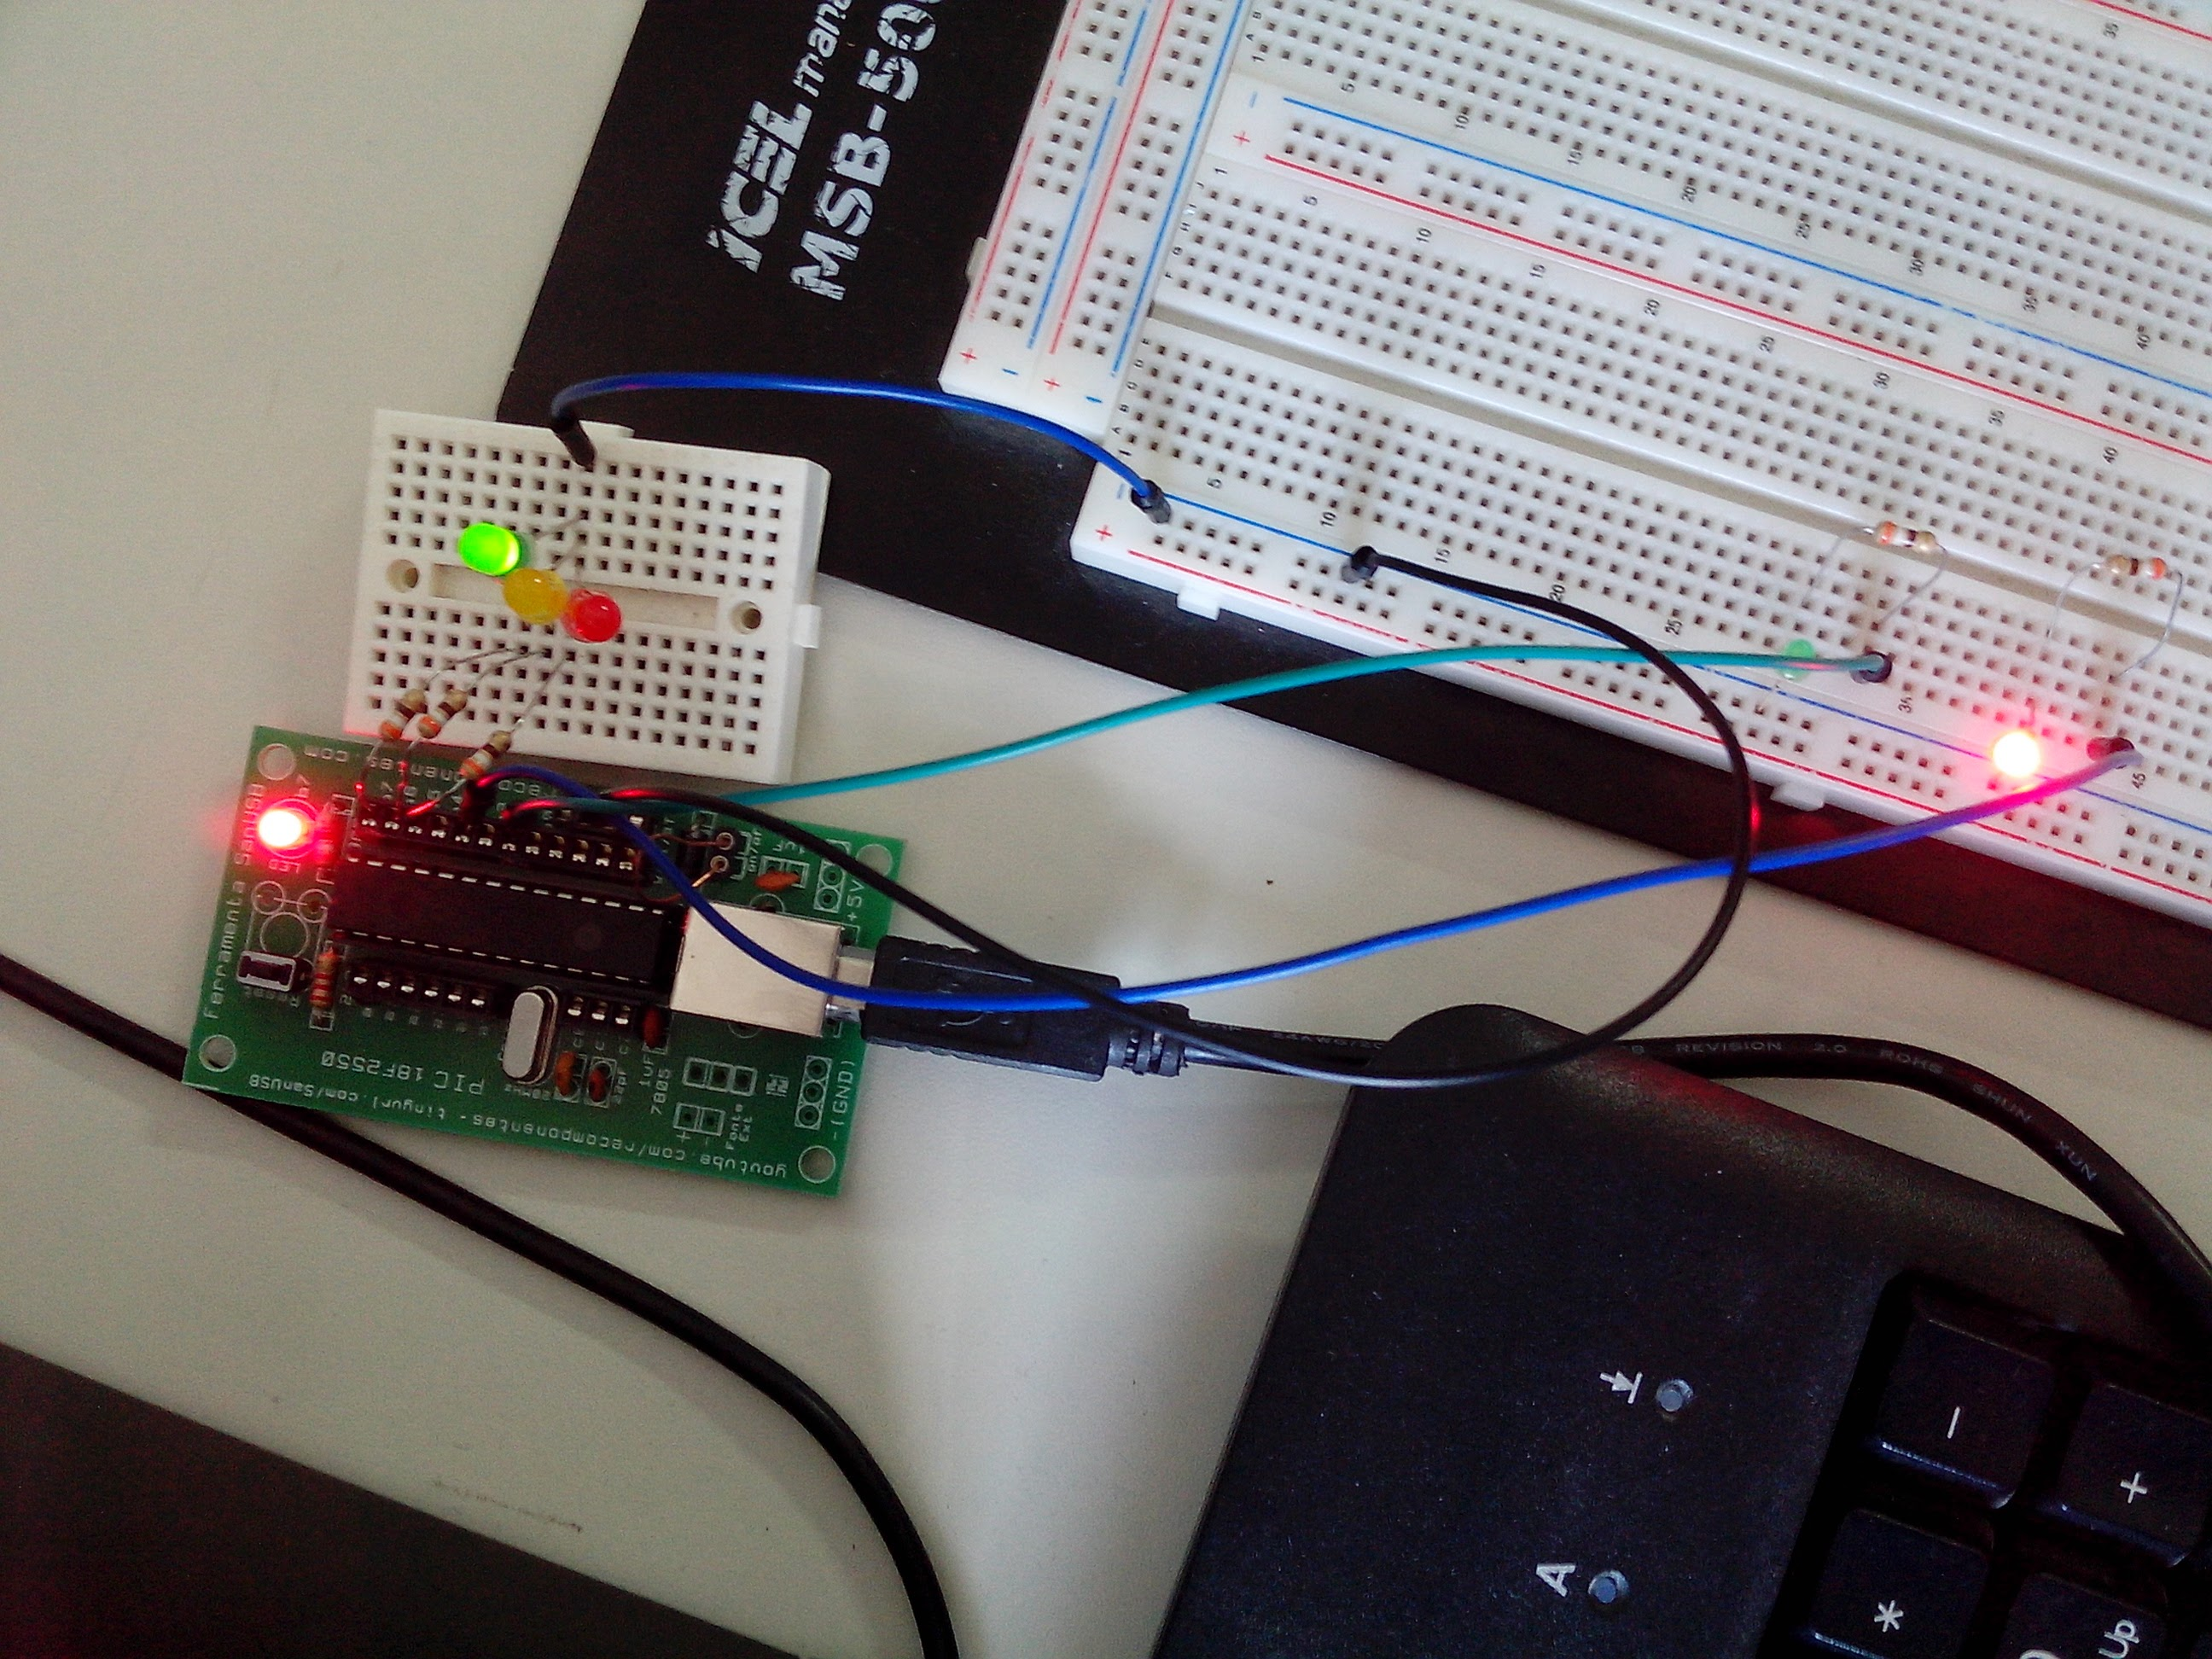
\includegraphics[scale=0.15]{img/semaforo-2.jpg}
    \caption{Semáforo simples para carros e pedestres}
\end{figure}

Segue o código fonte da iteração:

\begin{Shaded}
\begin{Highlighting}[]
\OtherTok{#include "SanUSB48X.h"}
\DataTypeTok{void} \NormalTok{interrupt interrupcao() \{\}}

\OtherTok{#define verde_carro pin_b7}
\OtherTok{#define amarelo_carro pin_b6}
\OtherTok{#define vermelho_carro pin_b5}

\OtherTok{#define vermelho_pedestre pin_b3}
\OtherTok{#define verde_pedestre pin_b1}

\DataTypeTok{int} \NormalTok{flag_pedestre = }\DecValTok{0}\NormalTok{, i;}

\DataTypeTok{void} \NormalTok{tempo(}\DataTypeTok{int} \NormalTok{tempo) \{}
    \KeywordTok{for} \NormalTok{(i = }\DecValTok{0}\NormalTok{; i < tempo; i += }\DecValTok{100}\NormalTok{) \{}
        \NormalTok{tempo_ms(}\DecValTok{100}\NormalTok{);}
        \KeywordTok{if} \NormalTok{(! entrada_pin_e3) \{}
            \NormalTok{flag_pedestre = }\DecValTok{1}\NormalTok{;}
        \NormalTok{\}}
    \NormalTok{\}}
\NormalTok{\}}

\DataTypeTok{void} \NormalTok{main(}\DataTypeTok{void}\NormalTok{) \{}
    \NormalTok{clock_int_48MHz();}
        \KeywordTok{while} \NormalTok{(}\DecValTok{1}\NormalTok{) \{}
        \NormalTok{nivel_alto(vermelho_pedestre);}
        \NormalTok{nivel_baixo(vermelho_carro);}

        \NormalTok{nivel_alto(verde_carro);}
        \NormalTok{tempo(}\DecValTok{10000}\NormalTok{);}
        \NormalTok{nivel_baixo(verde_carro);}

        \KeywordTok{if} \NormalTok{(flag_pedestre) \{}
            \NormalTok{nivel_alto(amarelo_carro);}
            \NormalTok{tempo_ms(}\DecValTok{1000}\NormalTok{);}
            \NormalTok{nivel_baixo(amarelo_carro);}

            \NormalTok{nivel_alto(vermelho_carro);}
            \NormalTok{nivel_baixo(vermelho_pedestre);}

            \NormalTok{nivel_alto(verde_pedestre);}
            \NormalTok{tempo_ms(}\DecValTok{5000}\NormalTok{);}
            \NormalTok{nivel_baixo(verde_pedestre);}
            \NormalTok{flag_pedestre = }\DecValTok{0}\NormalTok{;}
        \NormalTok{\}}
    \NormalTok{\}}
\NormalTok{\}}
\end{Highlighting}
\end{Shaded}
\newpage

\section{Iteração 3 - Display de 7 segmentos com contagem regressiva}

Agora que temos um semáforo precisaremos usar um display de 7 segmentos
que irá mostrar a contagem regressiva para que o sinal verde do pedestre
vá para vermelho. Mas antes vamos fazer apenas que o display conte de
zero a nove indefinidamente.

\begin{figure}[H]
    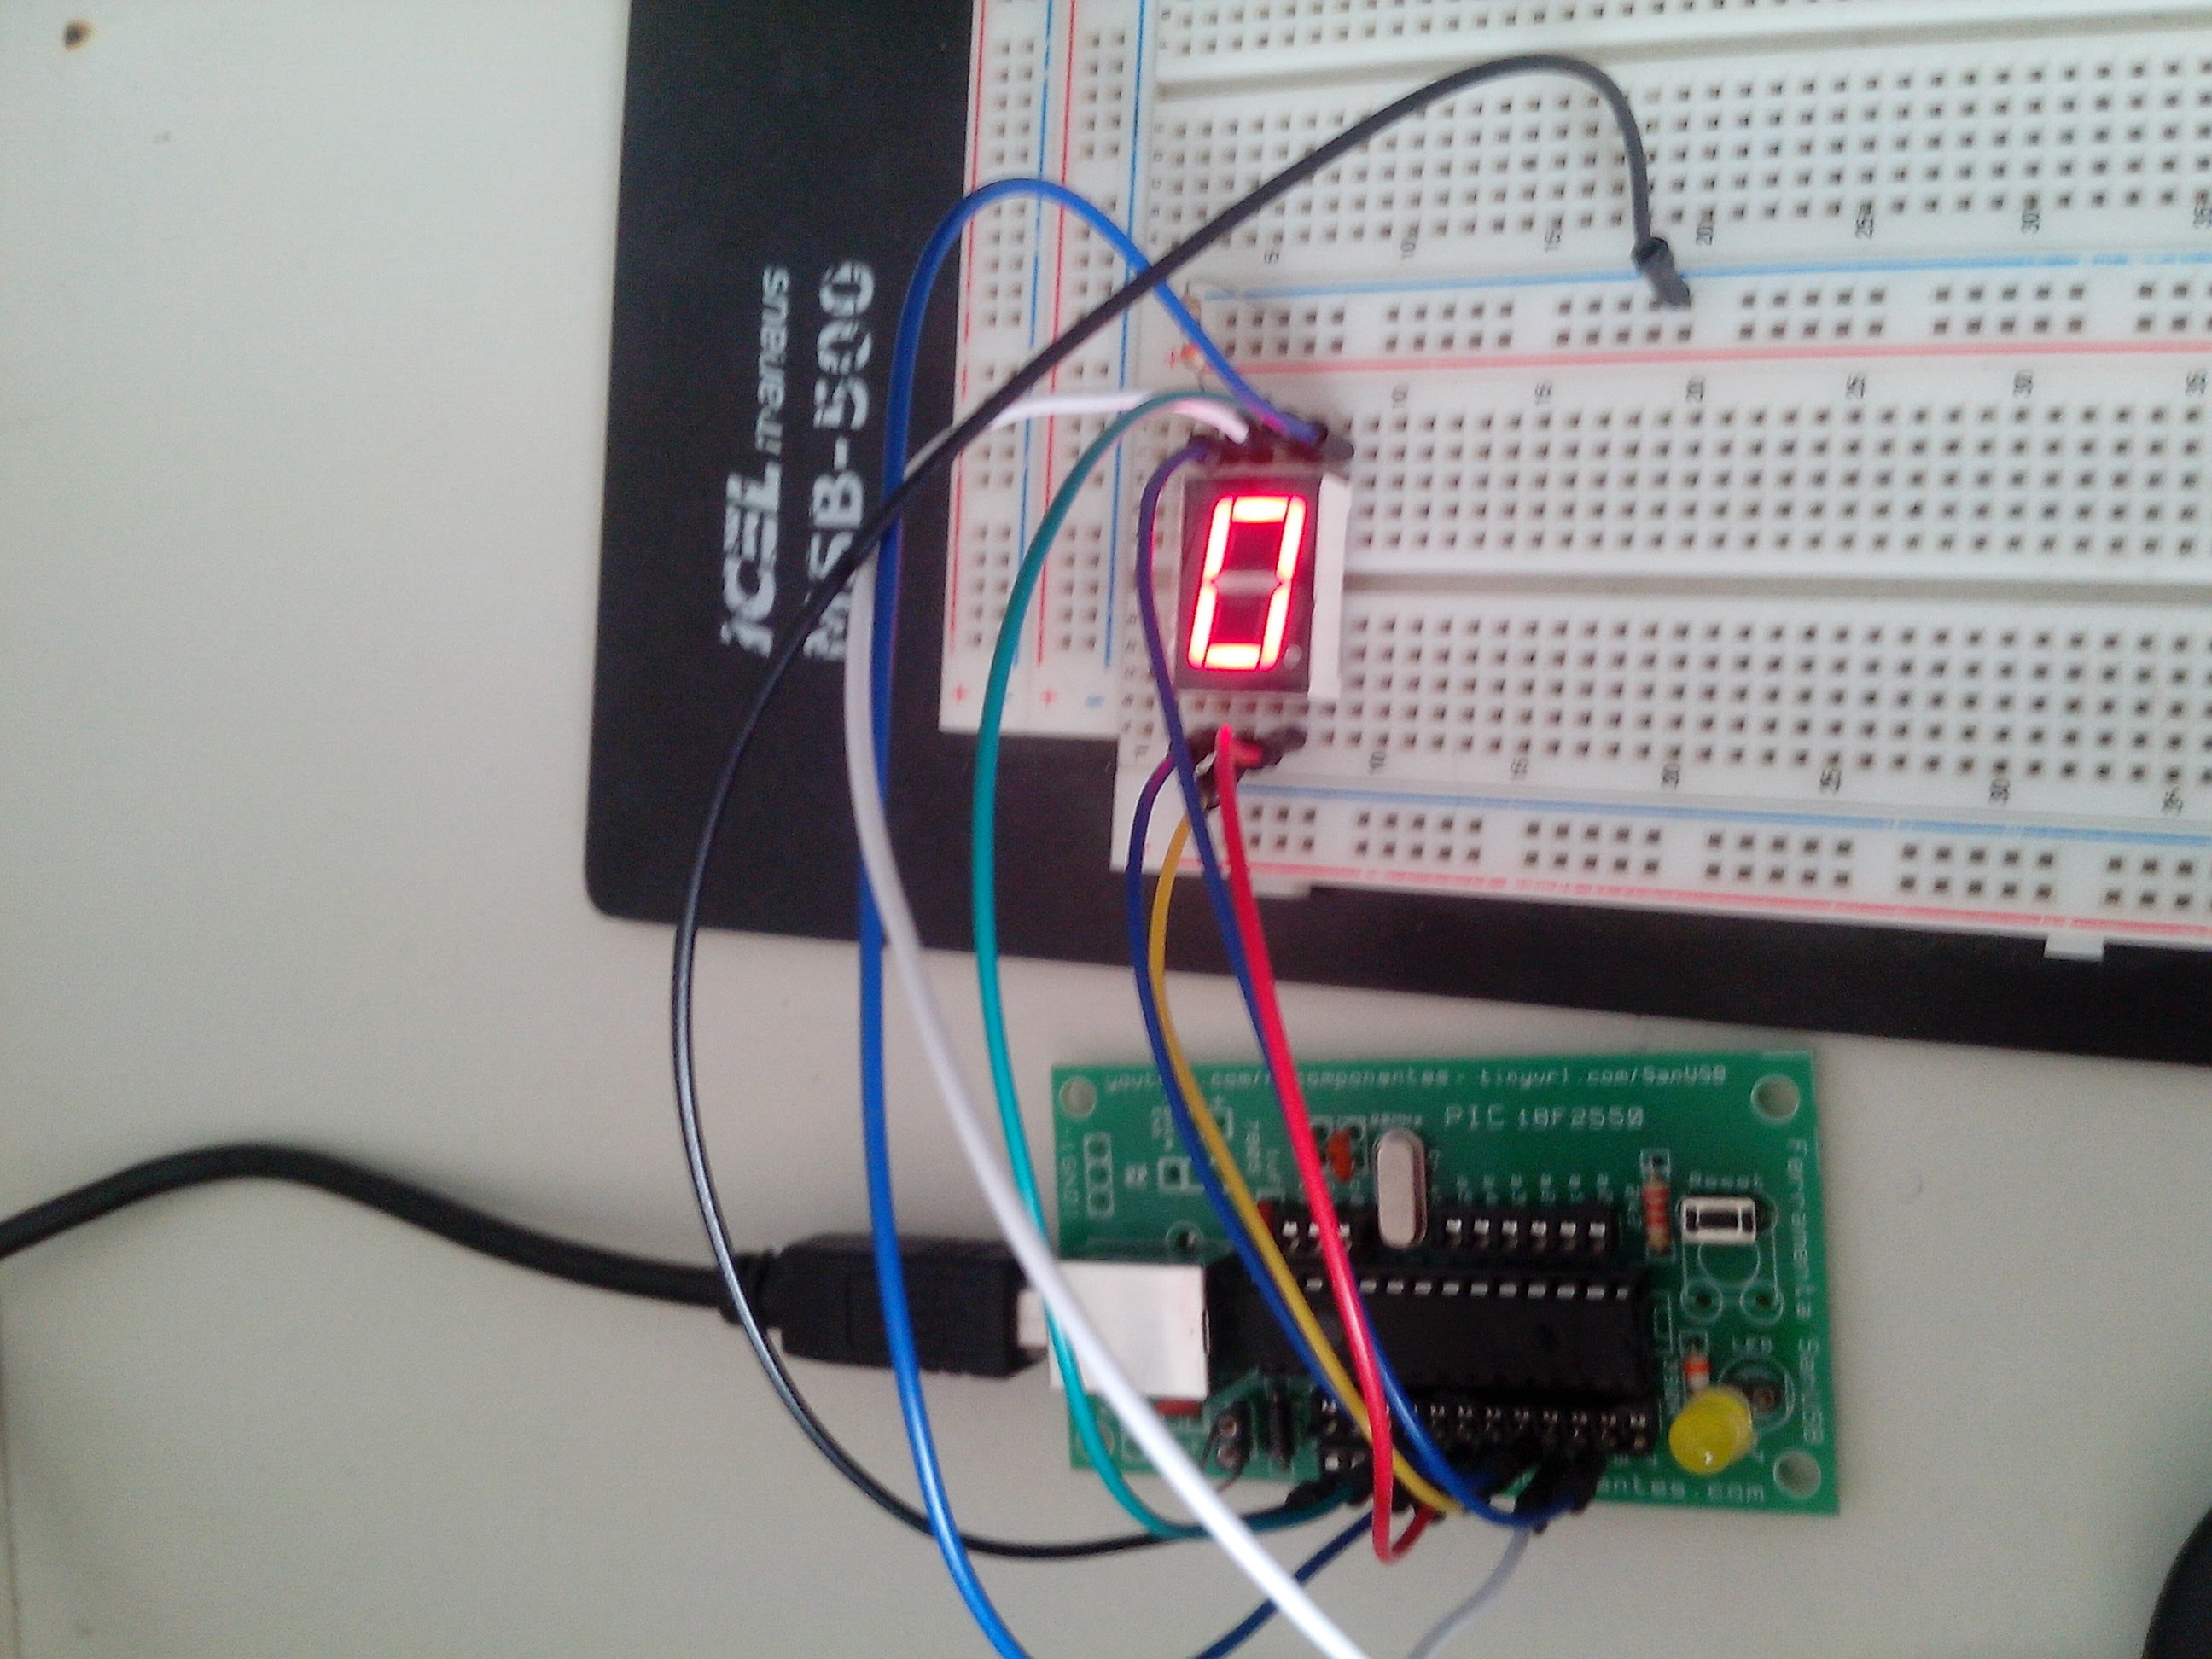
\includegraphics[scale=0.15]{img/display-7seg-1.jpg}
    \caption{Display de 7 segmentos com contagem regressiva}
\end{figure}
